% Created 2018-11-07 Wed 21:28
% Intended LaTeX compiler: pdflatex
\documentclass[table]{article}
\usepackage[utf8]{inputenc}
\usepackage[T1]{fontenc}
\usepackage{graphicx}
\usepackage{grffile}
\usepackage{longtable}
\usepackage{wrapfig}
\usepackage{rotating}
\usepackage[normalem]{ulem}
\usepackage{amsmath}
\usepackage{textcomp}
\usepackage{amssymb}
\usepackage{capt-of}
\usepackage{hyperref}
\usepackage{amsmath}
\usepackage[usenames]{color}
\usepackage{pstricks}
\usepackage{pgfplots}
\pgfplotsset{compat=1.8}
\usepackage{tikz}
\usepackage[europeanresistors,americaninductors]{circuitikz}
\usepackage{colortbl}
\usepackage{yfonts}
\usetikzlibrary{shapes,arrows}
\usetikzlibrary{positioning}
\usetikzlibrary{arrows,shapes}
\usetikzlibrary{intersections}
\usetikzlibrary{calc,patterns,decorations.pathmorphing,decorations.markings}
\usepackage[BoldFont,SlantFont,CJKchecksingle]{xeCJK}
\setCJKmainfont[BoldFont=Evermore Hei]{Evermore Kai}
\setCJKmonofont{Evermore Kai}
\xeCJKsetup{CJKglue=\hspace{0pt plus .08 \baselineskip }}
\usepackage{pst-node}
\usepackage{pst-plot}
\psset{unit=5mm}
\usepackage{beamerarticle}
\mode<beamer>{\usetheme{Frankfurt}}
\mode<beamer>{\usecolortheme{dove}}
\mode<article>{\hypersetup{colorlinks=true,pdfborder={0 0 0}}}
\mode<beamer>{\AtBeginSection[]{\begin{frame}<beamer>\frametitle{Topic}\tableofcontents[currentsection]\end{frame}}}
\setbeamercovered{transparent}
\subtitle{频域稳定性判据}
\date{}
\title{线性系统的频域分析法}
\hypersetup{
 pdfauthor={},
 pdftitle={线性系统的频域分析法},
 pdfkeywords={},
 pdfsubject={},
 pdfcreator={Emacs 26.1 (Org mode 9.1.9)}, 
 pdflang={English}}
\begin{document}

\maketitle
\tableofcontents











\section{Nyquist稳定性判据}
\label{sec:org62a7efa}
\subsection{辐角原理}
\label{sec:org77da4cb}
\begin{itemize}
\item 设  \(s\)  为复变量,  \(F(s)\)  为  \(s\)  的有理分式函数.对于  \(s\)  平面上任意一点  \(s\)  , 通过复变函数  \(F(s)\)  的映射关系,可以确定  \(s\)  的象.
\item 在  \(s\)  平面上任选一条闭合曲线  \(\Gamma\)  ,且不通过  \(F(s)\)  任一零点和极点,  \(s\)  沿闭合曲线  \(\Gamma\)  运动一周,则相应地  \(F(s)\)  形成一条闭合曲线  \(\Gamma_F\) .
\end{itemize}
\subsection{辐角原理(续):}
\label{sec:orgb7bcbb0}
设  \(s\)  平面闭合曲线  \(\Gamma\)  包围  \(F(s)\)  的  \(Z\)  个零点和  \(P\)  个极点,则  \(s\)  沿  \(\Gamma\)  顺时针运动一周时,在  \(F(s)\)  平面上,  \(F(s)\)  沿闭合曲线  \(\Gamma_F\)  逆时针包围原点的圈数为  \(R=P-Z\) .

\begin{tikzpicture}
\draw[->] (-1,0) -- (4.5,0);
\draw[->] (0,-2) -- (0,2);
\draw (0,2) node[above left] {$j$};
\draw (2,2) node[above right] {$\Gamma$};
%\draw[dashed] (-4,-5) -- (-4,0);
\draw [red] plot [smooth] coordinates {(1,0.5) (2,2)  (3,1.5) (3.5,0) (1.1,0) (1,0.5)};
\draw (1,0.5) node {$\cdot$};
\draw (1,0.5) node[left] {$s$};
\draw[blue,->,thick] (1,0.5)-- ++(0.3,0.6);
\draw (2,1) node {$\times$};
\draw (2,-1) node {$\times$};
\draw (2.3,0) node {$\times$};
\draw (2.7,0.3) node {$\circ$};
\draw (2.7,-0.3) node {$\circ$};

\begin{scope}[shift={(7,0)}]
\draw[->] (-2,0) -- (2,0);
\draw[->] (0,-2) -- (0,2);
\draw (0,2) node[above left] {$j$};
\draw (1,1) node[above right] {$\Gamma_F$};
\draw[red] (0,0) ++(0:1) arc (0:360:1);
\draw[thick] (120:1) node {$\cdot$};
\draw (120:1) node[above left] {$F(s)$};
\draw (0,0) node[below left] {$o$};
\draw[blue,->,thick] (120:1)-- ++(-0.3,-0.2);
\end{scope}
\end{tikzpicture}

\subsection{辐角原理的应用}
\label{sec:org3a81c8a}
\begin{eqnarray*}
\Phi(s) &= &\frac{G(s)}{1+G(s)H(s)} \\
       &=&\frac{G(s)}{1+G_o(s)} \\
       &=&\frac{G(s)}{F(s)} \\
 F(s)&=&1+G_o(s)
\end{eqnarray*}
\begin{itemize}
\item \(F(s)\)  的极点是系统开环极点,
\item \(F(s)\)  的零点是系统的闭环极点.
\end{itemize}

\subsection{辐角原理的应用(续)}
\label{sec:org06f397c}
\subsubsection[示意图]{示意图\hfill{}\textsc{B\_ignoreheading:BMCOL}}
\label{sec:org7b3c5b9}
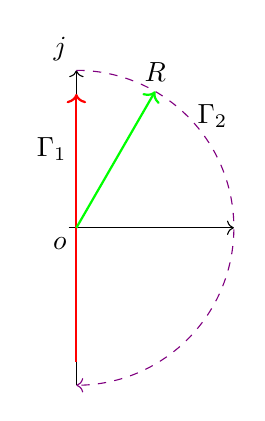
\begin{tikzpicture}
\draw[->] (-0.1,0) -- (2,0);
\draw[->] (0,-2) -- (0,2);
\draw (0,2) node[above left] {$j$};
\draw (0,0) node[below left] {$o$};
\draw[red,thick,->] (0,-1.7) -- (0,1.7);
\draw[violet,dashed,->] (0,2) arc (90:-90:2);
\draw[green,thick,->] (0,0) -- (60:2);
\draw (60:2) node[above] {$R$};
\draw (0,1) node[left] {$\Gamma_1$};
\draw (45:2) node[right] {$\Gamma_2$};
\end{tikzpicture}

\subsubsection[将 \(\Gamma\) 分为两段:]{将 \(\Gamma\) 分为两段:\hfill{}\textsc{BMCOL:B\_block}}
\label{sec:org3060a3d}
\begin{itemize}
\item \(\Gamma_1\) : \(s=j\omega,\omega\in[-\infty,\infty]\)
\item \(\Gamma_2\) : \(s=\lim_{R\rightarrow\infty}Re^{j\theta}\) , \(\theta\) 从 \(\frac{\pi}{2}\) 到 \(-\frac{\pi}{2}\)
\item 可得对应的 \(G_o(s)\) 曲线.
\begin{itemize}
\item \(s\) 在 \(\Gamma_1\) 上时,与Nyquist图对应.(\(\omega\in[0,\infty]\))
\item \(s\) 在 \(\Gamma_1\) 上时, \(F(s)=1+G_o(s)=1+\lim_{R\rightarrow\infty}Re^{j\theta}G_o(s)=1\)
\end{itemize}
\item <3-> Nyquist判据
\begin{itemize}
\item 对于开环稳定系统(\(P=0\)),若Nyquist曲线不包含 \((-1,0)\) 点,则系统稳定.
\item 对于开环不稳定系统(\(P>0\)),若Nyquist曲线逆时针包围 \((-1,0)\) 点的次数为 \(\frac{P}{2}\) ,则系统稳定.
\end{itemize}
\end{itemize}

\subsection{Nyquist判据,例1:}
\label{sec:org083180e}
某负反馈开环传递函数为 \(G_o(s)=\frac{10}{s-1}\) ,用Nyquist判据判断系统稳定性.

\subsubsection[Nyquist图]{Nyquist图\hfill{}\textsc{BMCOL:B\_block}}
\label{sec:org25f467f}
\begin{tikzpicture}[scale=0.5]
%g=10/(s-1)
\begin{axis}[
%axis x line=middle,axis y line= middle, 
ylabel=$j$ ,xlabel=$   $ ,
ymin=-5.7,ymax=1,xmin=-11,xmax=1,every axis plot post/.append style={mark=none},
grid=both]
\addplot[blue,thick,->]
shell {
octave -q --eval "s=tf('s');g=10/(s-1);[re,im]=nyquist(g);disp([re,im]);"
};
\end{axis}
\end{tikzpicture}

\subsubsection[稳定性判断]{稳定性判断\hfill{}\textsc{BMCOL:B\_block}}
\label{sec:orgcaf72e2}
\begin{eqnarray*}
P & = & 1\\
N &=& \frac{1}{2} \\
P-Z &=& 2N \\
Z &=& P-2N \\
  &=&0 
\end{eqnarray*}
系统稳定.

\subsection{虚轴上有极点时}
\label{sec:org91d5ddd}
\begin{itemize}
\item 零型系统 \(F(s)\) 沿 \(\Gamma\) 解析且不为0.
\item I型及以上系统 \(F(s)\) 在 \(s=0\) 处不解析,不满足辐角原理条件.
\end{itemize}

\subsubsection[示意图]{示意图\hfill{}\textsc{B\_ignoreheading:BMCOL}}
\label{sec:org0ba107e}
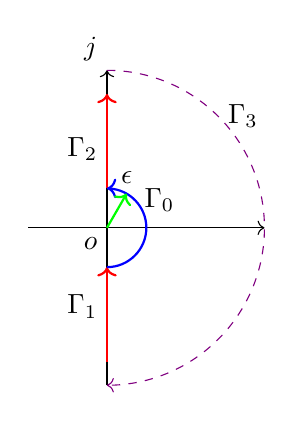
\begin{tikzpicture}
\draw[->] (-1,0) -- (2,0);
\draw[->] (0,-2) -- (0,2);
\draw (0,2) node[above left] {$j$};
\draw (0,0) node[below left] {$o$};
\draw[red,thick,->] (0,0.5) -- (0,1.7);
\draw[red,thick,->] (0,-1.7) -- (0,-0.5);
\draw[blue,thick,->] (0,0)++(-90:0.5) arc (-90:90:0.5);
\draw[violet,dashed,->] (0,2) arc (90:-90:2);
\draw[green,thick,->] (0,0) -- (60:0.5);
\draw (60:0.5) node[above] {$\epsilon$};
\draw (0,1) node[left] {$\Gamma_2$};
\draw (45:0.5) node[right] {$\Gamma_0$};
\draw (0,-1) node[left] {$\Gamma_1$};
\draw (45:2) node[right] {$\Gamma_3$};
\end{tikzpicture}

\subsubsection[将 \(\Gamma\) 分为四段:]{将 \(\Gamma\) 分为四段:\hfill{}\textsc{BMCOL:B\_block}}
\label{sec:org823a2e7}
\begin{itemize}
\item \(\Gamma_1\) : \(s=j\omega,\omega\in[-\infty,0^-]\)
\item \(\Gamma_2\) : \(s=j\omega,\omega\in[0^+,\infty]\)
\item \(\Gamma_3\) : \(s=\lim_{R\rightarrow\infty}Re^{j\theta},\theta\in[-\frac{\pi}{2},\frac{\pi}{2}]\)
\item \(\Gamma_0\) : \(s=\lim_{\epsilon\rightarrow 0}\epsilon e^{j\theta},\theta\in[-\frac{\pi}{2},\frac{\pi}{2}]\)
\item <3->对增补后的Nyquist图可使用Nyquist判据.
\end{itemize}

\subsection{穿越次数}
\label{sec:org62c5a74}
\subsubsection[Nyquist图]{Nyquist图\hfill{}\textsc{BMCOL:B\_block}}
\label{sec:org79d93fc}
\begin{tikzpicture}[scale=0.5]
\begin{axis}[
axis x line=middle,axis y line= middle, 
ylabel=$j$ ,xlabel=$   $ ,
ymin=-2.5,ymax=1,xmin=-3.5,xmax=3.5,every axis plot post/.append style={mark=none}]
grid=both,
\addplot[smooth,blue,thick,->]
shell {
octave -q --eval "
a=[0.01 3   0;
   0.1  0   -2; 
   1   -3   0; 
   2   -2.3  0.5; 3 -1.7 0; 4 -1 -0.5; 3 -0.5 0 ;5 -0.25 0.25; 7 0 0];
disp(a(:,2:3));"};
\end{axis}
\end{tikzpicture}

\subsubsection[穿越次数]{穿越次数\hfill{}\textsc{BMCOL:B\_block}}
\label{sec:orgbb0f696}
\begin{itemize}
\item 根据增补后的Nyquist曲线穿越 \((-1,0)\) 点左侧的次数可得 \(\Gamma_F\) 包围原点的圈数
\begin{eqnarray*}
R &=  &2N \\
  &=& 2(N_+ - N_-)
\end{eqnarray*}
其中,
\begin{itemize}
\item \(N_+\) 为正穿越(自上向下)次数
\item \(N_-\) 为负穿越(自下向上)次数
\end{itemize}
\end{itemize}

\subsection{例: \(G_o(s)=\frac{10}{s(s+1)}\)}
\label{sec:org7b2faee}

\begin{tikzpicture}
%g=10/s/(s+1)
\begin{axis}[
axis x line=middle,axis y line= middle, 
ylabel=$j$ ,xlabel=$   $ ,
ymin=-9,ymax=1,xmin=-6,xmax=10,every axis plot post/.append style={mark=none}]
grid=both,
\addplot[blue,thick,->]
shell {
octave -q --eval "s=tf('s');g=10/s/(s+1);[re,im]=nyquist(g);disp([re,im]);"
};
\addplot[red,dashed,->]shell {octave -q --eval "t=[-0.1:-0.1:-pi*1.5/2]';disp(8*[cos(t),sin(t)]);"};
\end{axis}
\end{tikzpicture}

\section{Bode稳定性判据}
\label{sec:org7ffc141}
\subsection{Bode稳定性判据}
\label{sec:orgd2ad7d9}
\subsubsection[Bode图]{Bode图\hfill{}\textsc{BMCOL:B\_ignoreheading}}
\label{sec:org96d6ad5}
\begin{tikzpicture}[scale=0.42]
\begin{semilogxaxis}[
%axis x line=middle,axis y line= left, 
ylabel=$L(\omega)/L_a(\omega)$ ,xlabel=$\omega$ ,
every axis plot post/.append style={mark=none},
grid=both,
ymin=-10,ymax=20,xmin=0.01,xmax=10]
\addplot[smooth,blue,thick]
 shell {
octave -q --eval "
a=[0.01 3   0;
   0.1  0   -2; 
   1   -3   0; 
   2   -2.3  0.5; 
   3 -1.7 0;
   5 -1 -0.5;
   7 -0.5 0 ;
   10 -0.25 0.25];
w=a(:,1);
a=a(:,2)+i*a(:,3);
m=abs(a);
disp([w,20*log(m)/log(10)]);"};
\end{semilogxaxis}
\end{tikzpicture}
\begin{tikzpicture}[scale=0.42]
\begin{semilogxaxis}[
%axis x line=middle,axis y line= left, 
ylabel=$\phi(\omega)$ ,xlabel=$\omega$ ,
every axis plot post/.append style={mark=none},
grid=both,
ymin=-200,ymax=10,xmin=0.01,xmax=11]
%\draw[blue,thick] (axis cs:0.1,90)--(axis cs:10,90);
\addplot[smooth,blue,thick]
shell {
octave -q --eval "
a=[0.01 3   0;
   0.1  0   -2; 
   1   -3   0; 
   2   -2.3  0.5; 
   3 -1.7 0;
   5 -1 -0.5;
   7 -0.5 0 ;
   10 -0.25 0.25];
w=a(:,1);
a=a(:,2)+i*a(:,3);
p=angle(a)*180/pi;
p(p>0)=p(p>0)-360;
disp([w,p]);"};
\draw[red,dashed] (axis cs:0.01,-180) --(axis cs:10,-180);
\draw[red,dashed] (axis cs:5,-190) --(axis cs:5,-170);
\end{semilogxaxis}
\end{tikzpicture}
\begin{tikzpicture}[scale=0.42]
\begin{axis}[
%axis x line=middle,axis y line= middle, 
ylabel=$j$ ,xlabel=$   $ ,
ymin=-2.5,ymax=1,xmin=-3.5,xmax=3.5,every axis plot post/.append style={mark=none},
grid=both]
\addplot[smooth,blue,thick,->]
shell {
octave -q --eval "
a=[0.01 3   0;
   0.1  0   -2; 
   1   -3   0; 
   2   -2.3  0.5; 3 -1.7 0; 4 -1 -0.5; 3 -0.5 0 ;5 -0.25 0.25; 7 0 0];
disp(a(:,2:3));"};
\end{axis}
\end{tikzpicture}

\subsubsection[稳定性判断]{稳定性判断\hfill{}\textsc{BMCOL:B\_block}}
\label{sec:org3326e55}
\begin{itemize}
\item 截止频率 \(\omega_c\) : \(A(\omega_c)=0\)
\item 穿越频率 \(\omega_x\) : \(\phi(\omega_x)=(2k+1)\pi\)
\item <3->Bode判据:
\begin{itemize}
\item 最小相位系统,若在 \(\omega<\omega_c\) 前 \(N_+-N_-=0\) ,则系统稳定
\item 非最小相位系统,若在 \(\omega<\omega_c\) 前 \(N_+-N_-=\frac{P}{2}\) ,则系统稳定
\end{itemize}
\end{itemize}
\end{document}